% ================================================================
% The printable version of latex/starters/targeted/KS3/algebra/expandingDoubleBracketsStarter_retrieveAndConnect.tex
%
% This is the same deck, laid out to be handed out rather than put on
% the board. Every slide is shown as it stands before any answer is
% revealed, and 4 copies of it go on one page of A4, two by two, so
% that a printed page cuts into four question sheets.
%
%   made from           latex/starters/targeted/KS3/algebra/expandingDoubleBracketsStarter_retrieveAndConnect.tex
%   slides on the sheet 2
%   slides left out     2 - a title slide, a contents slide, or a
%                       note meant for whoever maintains the deck
%   copies of each      4, two by two on A4 landscape
%   printing rules      version 1
%
% Nothing was reworded and nothing was rewritten. Each slide is the slide
% from the deck, asked for at its first step, which is how the answers
% stay hidden.
%
% Please don't edit this file. It is written again from the one it was
% made from whenever that changes, so an edit here would be lost - edit
% that file instead and this one follows.
% ================================================================
% ================================================================
% The Retrieve and Connect version of latex/starters/targeted/KS3/algebra/expandingDoubleBracketsStarter.tex
%
% This is the same deck as the one above, made by renaming the titles in it.
% Every slide that was a numbered starter is now titled
% "Retrieve and Connect", and the word is renamed wherever else a title
% used it. Nothing outside a title has been changed.
%
%   made from           latex/starters/targeted/KS3/algebra/expandingDoubleBracketsStarter.tex
%   retitling rules     version 1
%
% Please don't edit this file. It is written again from the one it was
% made from whenever that changes, so an edit here would be lost - edit
% that file instead and this one follows.
% ================================================================
\documentclass{beamer}
\usetheme{default} % You can swap theme if you like (e.g., Madrid, Boadilla)
\usepackage{tikz} 

% ================================================================
% Answer-overlay helpers
% ================================================================
\newcommand{\ablank}[1]{%
  \alt<2>{\textcolor{red}{#1}}{\underline{\phantom{#1}}}%
}
\newcommand{\ashow}[1]{\uncover<2->{\textcolor{red}{\small #1}}}
\newcommand{\ashowq}[1]{\alt<2->{\textcolor{red}{\small #1}}{?}}

% Answers drawn straight on to a TikZ diagram, revealed on overlay 2 like \ashow.
% Space is reserved on overlay 1, so the diagram does not move between slides.
\usetikzlibrary{overlay-beamer-styles}
\tikzset{
  ans/.style     = {red, thick, visible on=<2->},
  ansfill/.style = {red!15, visible on=<2->},
  anslab/.style  = {red, font=\tiny, visible on=<2->},
}

\title{Retrieve and Connect: Expanding Brackets}
\author{Year 8}
\date{}

% ---------------------------------------------------------------
% Added so this deck prints four slides to a page. Nothing above
% this line was changed.
% ---------------------------------------------------------------
\usepackage{pgfpages}

% 4 slides to a sheet of A4, two by two, with a thin line round each
% so that the page can be cut up. The margin is wide enough that the lines
% fall inside what a printer can actually put ink on.
\pgfpagesuselayout{4 on 1}[a4paper,landscape,border shrink=10mm]
\pgfpageslogicalpageoptions{1}{border code=\pgfusepath{stroke}}
\pgfpageslogicalpageoptions{2}{border code=\pgfusepath{stroke}}
\pgfpageslogicalpageoptions{3}{border code=\pgfusepath{stroke}}
\pgfpageslogicalpageoptions{4}{border code=\pgfusepath{stroke}}

% There is nothing on paper to click, and a slide announcing a new section
% would sit between two copies of the same question and put every page after
% it out of step with the grid.
\setbeamertemplate{navigation symbols}{}
\AtBeginPart{}
\AtBeginSection{}
\AtBeginSubsection{}
\AtBeginSubsubsection{}
\begin{document}



% ---------- STARTER (2x2 layout) ----------
\begin{frame}<1>{Retrieve and Connect: Expand each expression}
% Option A: simple 2x2 grid using minipages (consistent spacing)
\begin{minipage}[t]{0.48\textwidth}
  \begin{block}{1) Single brackets}
    \Large \(\;3(y+5)=\ablank{3y+15}\)
  \end{block}
  \vspace{0.5em}
  \begin{block}{3) Double brackets}
    \Large \(\;(x+4)(x-2)=\ablank{x^2+2x-8}\)
  \end{block}
\end{minipage}\hfill
\begin{minipage}[t]{0.48\textwidth}
  \begin{block}{2) Single brackets}
    \Large \(\; a(b-5)=\ablank{ab-5a}\)
  \end{block}
  \vspace{0.5em}
  \begin{block}{4) What is the area of the rectangle?}
    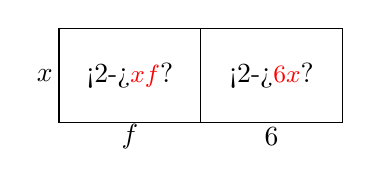
\begin{tikzpicture}[scale=0.6]

% Outer rectangle
\draw (0,0) rectangle (6,2);

% Vertical split
\draw (3,0) -- (3,2);

% Labels for widths
\node at (1.5,-0.3) {$f$};
\node at (4.5,-0.3) {$6$};

% Height label
\node at (-0.3,1) {$x$};

% Area labels
\node at (1.5,1) {\ashowq{$xf$}};
\node at (4.5,1) {\ashowq{$6x$}};

\end{tikzpicture}
    \par\vspace{0.5em}
    \ashow{Area = \(x(f+6)\)}
  \end{block}
\end{minipage}
\end{frame}
\begin{frame}<1>{Retrieve and Connect: Expand each expression}
% Option A: simple 2x2 grid using minipages (consistent spacing)
\begin{minipage}[t]{0.48\textwidth}
  \begin{block}{1) Single brackets}
    \Large \(\;3(y+5)=\ablank{3y+15}\)
  \end{block}
  \vspace{0.5em}
  \begin{block}{3) Double brackets}
    \Large \(\;(x+4)(x-2)=\ablank{x^2+2x-8}\)
  \end{block}
\end{minipage}\hfill
\begin{minipage}[t]{0.48\textwidth}
  \begin{block}{2) Single brackets}
    \Large \(\; a(b-5)=\ablank{ab-5a}\)
  \end{block}
  \vspace{0.5em}
  \begin{block}{4) What is the area of the rectangle?}
    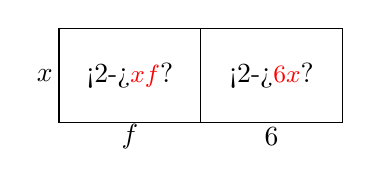
\begin{tikzpicture}[scale=0.6]

% Outer rectangle
\draw (0,0) rectangle (6,2);

% Vertical split
\draw (3,0) -- (3,2);

% Labels for widths
\node at (1.5,-0.3) {$f$};
\node at (4.5,-0.3) {$6$};

% Height label
\node at (-0.3,1) {$x$};

% Area labels
\node at (1.5,1) {\ashowq{$xf$}};
\node at (4.5,1) {\ashowq{$6x$}};

\end{tikzpicture}
    \par\vspace{0.5em}
    \ashow{Area = \(x(f+6)\)}
  \end{block}
\end{minipage}
\end{frame}
\begin{frame}<1>{Retrieve and Connect: Expand each expression}
% Option A: simple 2x2 grid using minipages (consistent spacing)
\begin{minipage}[t]{0.48\textwidth}
  \begin{block}{1) Single brackets}
    \Large \(\;3(y+5)=\ablank{3y+15}\)
  \end{block}
  \vspace{0.5em}
  \begin{block}{3) Double brackets}
    \Large \(\;(x+4)(x-2)=\ablank{x^2+2x-8}\)
  \end{block}
\end{minipage}\hfill
\begin{minipage}[t]{0.48\textwidth}
  \begin{block}{2) Single brackets}
    \Large \(\; a(b-5)=\ablank{ab-5a}\)
  \end{block}
  \vspace{0.5em}
  \begin{block}{4) What is the area of the rectangle?}
    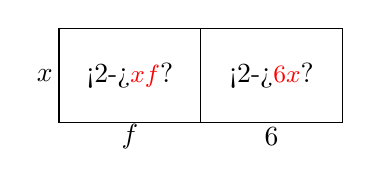
\begin{tikzpicture}[scale=0.6]

% Outer rectangle
\draw (0,0) rectangle (6,2);

% Vertical split
\draw (3,0) -- (3,2);

% Labels for widths
\node at (1.5,-0.3) {$f$};
\node at (4.5,-0.3) {$6$};

% Height label
\node at (-0.3,1) {$x$};

% Area labels
\node at (1.5,1) {\ashowq{$xf$}};
\node at (4.5,1) {\ashowq{$6x$}};

\end{tikzpicture}
    \par\vspace{0.5em}
    \ashow{Area = \(x(f+6)\)}
  \end{block}
\end{minipage}
\end{frame}
\begin{frame}<1>{Retrieve and Connect: Expand each expression}
% Option A: simple 2x2 grid using minipages (consistent spacing)
\begin{minipage}[t]{0.48\textwidth}
  \begin{block}{1) Single brackets}
    \Large \(\;3(y+5)=\ablank{3y+15}\)
  \end{block}
  \vspace{0.5em}
  \begin{block}{3) Double brackets}
    \Large \(\;(x+4)(x-2)=\ablank{x^2+2x-8}\)
  \end{block}
\end{minipage}\hfill
\begin{minipage}[t]{0.48\textwidth}
  \begin{block}{2) Single brackets}
    \Large \(\; a(b-5)=\ablank{ab-5a}\)
  \end{block}
  \vspace{0.5em}
  \begin{block}{4) What is the area of the rectangle?}
    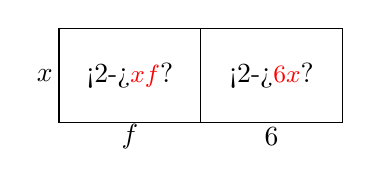
\begin{tikzpicture}[scale=0.6]

% Outer rectangle
\draw (0,0) rectangle (6,2);

% Vertical split
\draw (3,0) -- (3,2);

% Labels for widths
\node at (1.5,-0.3) {$f$};
\node at (4.5,-0.3) {$6$};

% Height label
\node at (-0.3,1) {$x$};

% Area labels
\node at (1.5,1) {\ashowq{$xf$}};
\node at (4.5,1) {\ashowq{$6x$}};

\end{tikzpicture}
    \par\vspace{0.5em}
    \ashow{Area = \(x(f+6)\)}
  \end{block}
\end{minipage}
\end{frame}

% ---------- ANSWERS ----------
\begin{frame}<1>{Answers}
\begin{enumerate}
  \item \(3(y+5)=3y+15\)
  \item \(a(b-5)=ab-5a\)
  \item \((x+4)(x-2)=x^2+2x-8\)
  \item Area = \(xf + 6x = x(f+6)\)
\end{enumerate}
\end{frame}
\begin{frame}<1>{Answers}
\begin{enumerate}
  \item \(3(y+5)=3y+15\)
  \item \(a(b-5)=ab-5a\)
  \item \((x+4)(x-2)=x^2+2x-8\)
  \item Area = \(xf + 6x = x(f+6)\)
\end{enumerate}
\end{frame}
\begin{frame}<1>{Answers}
\begin{enumerate}
  \item \(3(y+5)=3y+15\)
  \item \(a(b-5)=ab-5a\)
  \item \((x+4)(x-2)=x^2+2x-8\)
  \item Area = \(xf + 6x = x(f+6)\)
\end{enumerate}
\end{frame}
\begin{frame}<1>{Answers}
\begin{enumerate}
  \item \(3(y+5)=3y+15\)
  \item \(a(b-5)=ab-5a\)
  \item \((x+4)(x-2)=x^2+2x-8\)
  \item Area = \(xf + 6x = x(f+6)\)
\end{enumerate}
\end{frame}

% answer macro review note


\end{document}